\section{Profiling and Optimization}
In this section, I performed profiling and optimization on the IBP linear-Gaussian model. Profiling is done to identy the bottlenecks; the code structure can be visualized as a tree in Figure~\ref{fig:profiling}. In one Gibbs sampling iteration, generating $Z|\alpha$ and sampling $\sigma_X,\sigma_A$ are performed once each. In generating $Z|\alpha$, sampling dishes from $K_+$ and sampling new dishes are done for each customer (image or object), so they are each performed $N=100$ times. In sampling dishes from $K_+$, calculation refers to the process of sampling the posterior distribution of $Z|K_+$, and initialization is the part of removing features which are all zero. Both calculation and initialization are performed $N\times K_+ \approx 500$ times for each iteration.

\subsection{Profiling}
Table~\ref{tab:naive} shows the profiling results for my initial code. The calculation in sampling from $K_+$ for generating $Z|\alpha$ accounts for 70\% of the time, approximately 1.4 seconds per iteration because it involves matrix inversion and likelihood calculation.

\begin{figure}[!ht]
\centering
    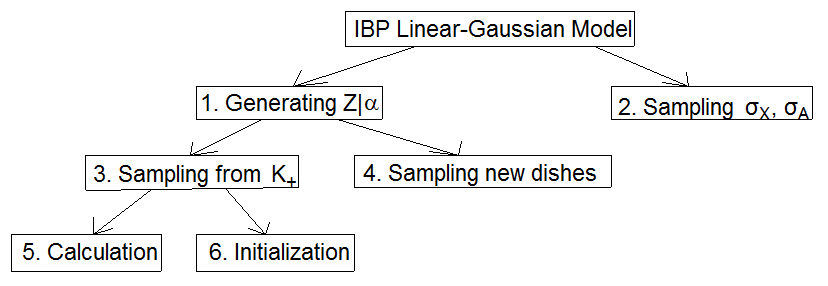
\includegraphics[width=\linewidth]{IBP_profiling.png}
    %\vspace{-20pt}
    \caption{IBP code structure for profiling}
    \label{fig:profiling}
\end{figure}

\subsection{Remove Redundant Calculations}
\label{sub:usable}
To optimize the code, redundant calculations are removed first, and this version is named as "usable". When generating $Z|\alpha$, the inverted matrix $\mathbf{M} = (\mathbf{Z}^T\mathbf{Z}+\frac{\sigma_X^2}{\sigma_A^2}\mathbf{I})^{-1}$ is only calculated directly before the likelihood computation, so more than $N = 100$ matrix inversions can be removed. The profiling results are shown in Table~\ref{tab:usable}. The "usable" version code can also be cythonized (converted from Python to C), and Table~\ref{tab:cythonized} is a summary of profiling results, but the Cythonized version only improved the speed about 0.5\%.

\subsection{Cythonized Code}
% Vectorization, calInverse
I also attempted to alleviate the bottleneck of calculating $\mathbf{M}$ by using Equations (51)-(54) in Griffiths' and Ghahramani's paper~\cite{griffiths2005detailed}, but this did not work because $K_+$ got stuck at 2. Theoretically, this method below allows us to efficiently compute $\mathbf{M}$ when only one $\mathbf{z_i}$ is changed:
\begin{gather}
\text{Define } \mathbf{M}_{-i} = (\sum_{j \neq i}\mathbf{z}^T_j \mathbf{z}_j + \frac{\sigma_X^2}{\sigma_A^2}\mathbf{I})^{-1} \\
\mathbf{M}_{-i} = (\mathbf{M}^{-1} - \mathbf{z}^T_i \mathbf{z}_i)^{-1} 
= \mathbf{M} - \dfrac{\mathbf{M}\mathbf{z}^T_i \mathbf{z}_i\mathbf{M}}{\mathbf{z}_i\mathbf{M}\mathbf{z}^T_i - 1} \\
\mathbf{M} = (\mathbf{M}_{-i}^{-1} - \mathbf{z}^T_i \mathbf{z}_i)^{-1} 
= \mathbf{M}_{-i} - \dfrac{\mathbf{M}_{-i}\mathbf{z}^T_i \mathbf{z}_i\mathbf{M}_{-i}}{\mathbf{z}_i\mathbf{M}_{-i}\mathbf{z}^T_i + 1}
\end{gather}
One drawback of this method is that numerical errors can be accumulated, leading to wrong results. Therefore, a full rank update of $\mathbf{M}$ should be performed occasionally.

\subsection{Using jit (just-in-time compiler)}

The jit (just-in-time compiler) is from the Python package \texttt{numba}, which generates optimized machine code from the LLVM compiler infrastructure. The jit in Python is claimed to have similar performance to C/C++ without switching languages~\cite{numba}. In fact, using jit (just-in-time compiler) to compile the $\mathbf{M}$ and log-likelihood calculation functions gives the best results of all four versions in speed. The execution time of generating $Z|\alpha$ is 7.5\% less than the initial code, and 5.2\% less than the "usable" version in Section~\label{sub:usable}. The speed comparison table is shown in Table~\ref{tab:jit}.

% Z|alpha: 7.5% improvement from the initial code, 5.2% improvement from the usable code.

\subsection{Comparison Tables}
All tables summarizing which actions take how much time are here for ease of comparison.

% A table to summarize which actions take how much time.
% Don't add minipage in front of tables!
\begin{table}[!ht]
  \centering
  \begin{tabular}{lrrr}
\toprule
{} &  Time (seconds)/action &  Times performed &  Total time (seconds) \\
\midrule
Generating Z given alpha &               1.598608 &                1 &              1.598608 \\
Sampling sigmaX, sigmaA  &               0.003846 &                1 &              0.003846 \\
Sampling from K+         &               0.011336 &              100 &              1.133637 \\
Sampling new dishes      &               0.004551 &              100 &              0.455109 \\
Calculation              &               0.002416 &              500 &              1.208202 \\
Initialization           &               0.000007 &              500 &              0.003707 \\
\bottomrule
\end{tabular}

  \caption{Initial code: Profiling results per iteration}
  \label{tab:naive}
\end{table}

\begin{table}[!ht]
  \centering
  \begin{tabular}{lrrr}
\toprule
{} &  Time (seconds)/action &  Times performed &  Total time (seconds) \\
\midrule
Generating Z given alpha &               1.962989 &                1 &              1.962989 \\
Sampling sigmaX, sigmaA  &               0.004164 &                1 &              0.004164 \\
Sampling from K+         &               0.014690 &              100 &              1.469040 \\
Sampling new dishes      &               0.004936 &              100 &              0.493605 \\
Calculation              &               0.002529 &              500 &              1.264704 \\
Initialization           &               0.000003 &              500 &              0.001566 \\
\bottomrule
\end{tabular}

  \caption{Usable code: Profiling results per iteration}
  \label{tab:usable}
\end{table}

\begin{table}[!ht]
  \centering
  \begin{tabular}{lrrr}
\toprule
{} &  Time (seconds)/action &  Times performed &  Total time (seconds) \\
\midrule
Generating Z given alpha &               1.951373 &                1 &              1.951373 \\
Sampling sigmaX, sigmaA  &               0.003792 &                1 &              0.003792 \\
Sampling from K+         &               0.014627 &              100 &              1.462701 \\
Sampling new dishes      &               0.004883 &              100 &              0.488332 \\
Calculation              &               0.002317 &              500 &              1.158574 \\
Initialization           &               0.000003 &              500 &              0.001499 \\
\bottomrule
\end{tabular}

  \caption{Cythonized code: Profiling results per iteration}
  \label{tab:cythonized}
\end{table}

\begin{table}[!ht]
  \centering
  \begin{tabular}{lrrr}
\toprule
{} &  Time (seconds)/action &  Times performed &  Total time (seconds) \\
\midrule
Generating Z given alpha &               1.859340 &                1 &              1.859340 \\
Sampling sigmaX, sigmaA  &               0.005764 &                1 &              0.005764 \\
Sampling from K+         &               0.013977 &              100 &              1.397660 \\
Sampling new dishes      &               0.004615 &              100 &              0.461481 \\
Calculation              &               0.002527 &              500 &              1.263748 \\
Initialization           &               0.000002 &              500 &              0.001063 \\
\bottomrule
\end{tabular}

  \caption{Using jit (just-in-time compiler): Profiling results per iteration}
  \label{tab:jit}
\end{table}